\documentclass[
 paper=A4,pagesize=automedia,fontsize=12pt,
 BCOR=15mm,DIV=22,
 twoside,headinclude,footinclude=false,
 ngerman,fleqn,             % fleqn = linksbündige Ausrichtung von Formeln
 bibtotocnumbered,          % Literaturverz. im Inhaltsverz. eintragen
 liststotoc,                % Abbildungsverz. im Inhaltsverz. eintragen
 listsleft,                 % Abbildungsverz. an der längsten Nummer ausrichten
 pointlessnumbers,          % kein Punkt nach Überschriftsnummerierung
 cleardoublepage=empty      % Vakatseiten ohne Paginierung
]{scrbook}
\setlength\parindent{0em}

% Kodierung, Schrift und Sprache auswählen
\usepackage[utf8]{inputenc}
\usepackage[T1]{fontenc}
\usepackage[ngerman]{babel}
% damit man Text aus dem PDF korrekt rauskopieren kann
\usepackage{cmap}
% Layout: Kopf-/Fußzeilen, anderthalbfacher Zeilenabstand
\usepackage{scrpage2} \pagestyle{scrheadings}
                      \clearscrheadfoot
                      \ihead{\headmark}\ohead{\pagemark}
                      \automark[subsection]{section}
                      \setheadsepline{0.5pt}
\usepackage{setspace} \onehalfspacing
\deffootnote{1em}{1em}{\textsuperscript{\thefootnotemark }}
% Grafiken, Tabellen, Mathematikumgebungen
\usepackage{graphicx,xcolor}
\usepackage{tabularx}
\usepackage{amsmath,amsfonts,amssymb}
% Darstellung von Fließumgebungen
\usepackage{flafter,afterpage}
\usepackage[section]{placeins}
\usepackage[margin=8mm,font=small,labelfont=bf,format=plain]{caption}
\usepackage[margin=8mm,font=small,labelfont=bf,format=plain]{subcaption}

\numberwithin{equation}{chapter}
\numberwithin{figure}{chapter}
\numberwithin{table}{chapter}

%%%%%%%%%%%%%%%%%%%%%%%%%%%%%%%%%%%%%%%%%%%%%%%%%%%%%%%%%%%%%%%%%%%%%%%%%%%%%%%%
% Ab hier ist Platz für eigene Ergänzungen (Pakete, Befehle, etc.)
%\usepackage{natbib}
%\usepackage{babelbib}
\DeclareUnicodeCharacter{2212}{-}
\newcommand{\gq}[1]{\glq#1\grq}
\newcommand{\gqq}[1]{\glqq#1\grqq}
\newcommand{\eq}[1]{`#1'}
\newcommand{\eqq}[1]{``#1''}
\usepackage{nicefrac}
\usepackage[style=alphabetic,backend=biber]{biblatex}
\addbibresource{bachref.bib}
\usepackage{graphicx,newfloat}
\usepackage[format=hang]{caption}
\DeclareCaptionType{InfoBox}
\usepackage{enumitem}
\usepackage[most]{tcolorbox}
\newcommand*\diff{\mathop{}\!\mathrm{d}}        % für schöne
\newcommand*\Diff[1]{\mathop{}\!\mathrm{d^#1}}  % Differenzialoperatoren
\usepackage{bigints}                            % große Integrale
\usepackage{float}

\begin{document}


\title{Fontsize Test}
\author{Max}
\maketitle
Normale Schriftgröße im ganzen Dokument.
\begin{figure}[H]
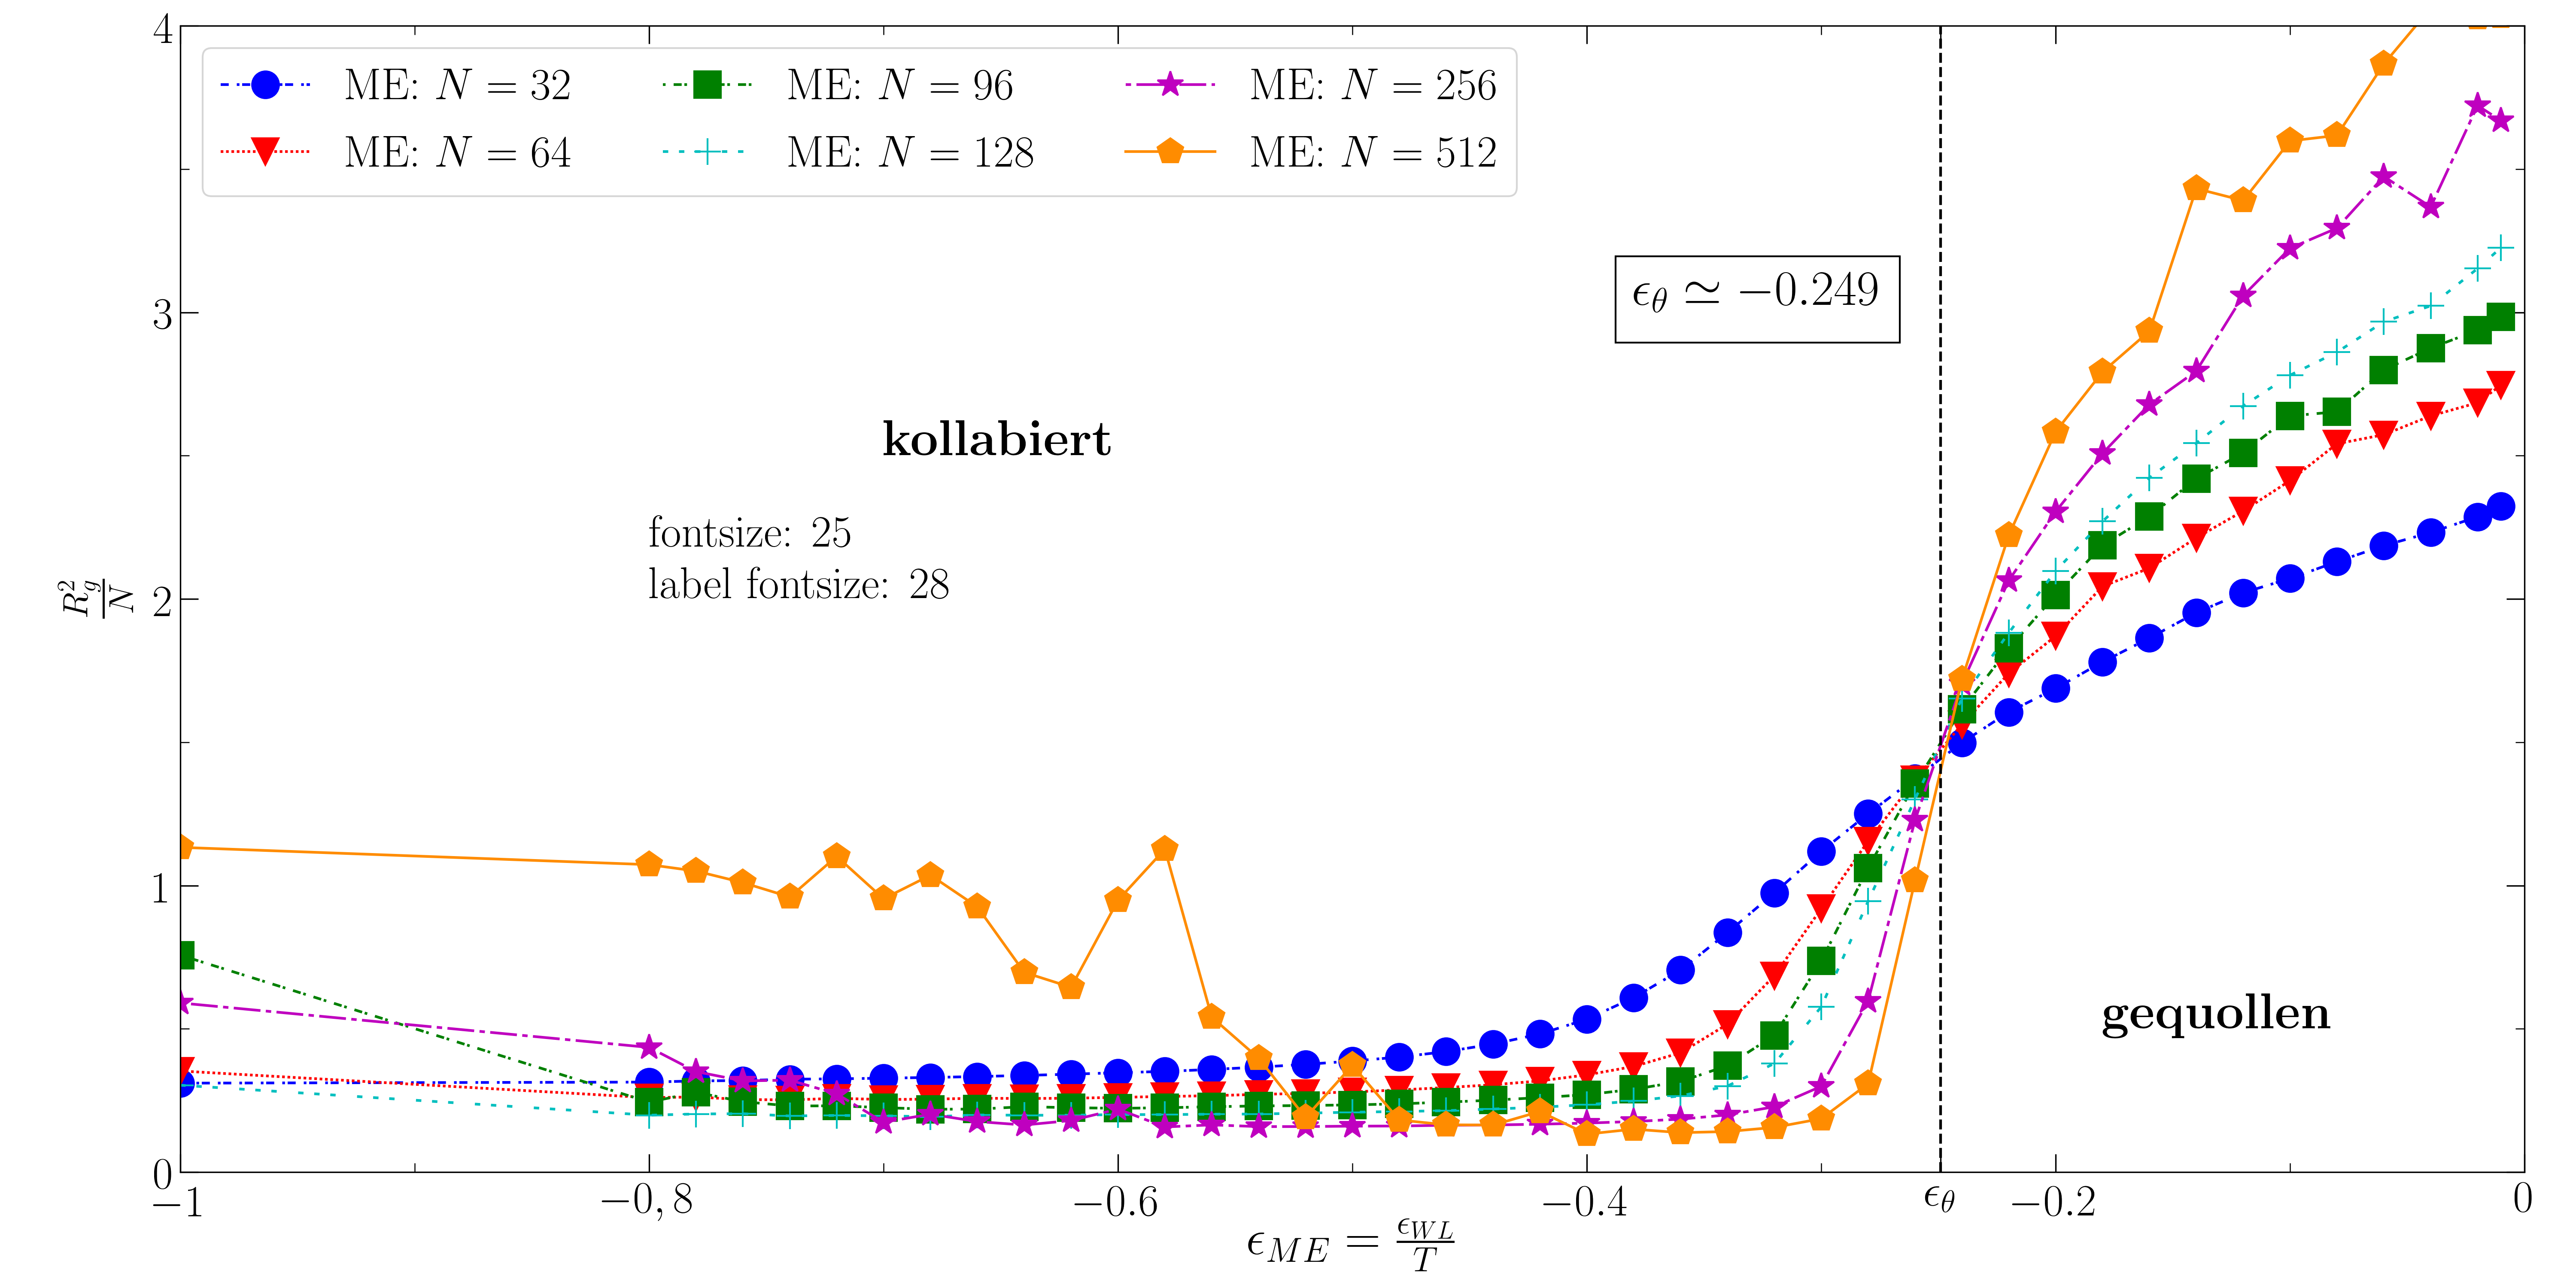
\includegraphics[width=\textwidth]{png_25_28.png}
\caption{Beschreibung des Bildes zum Größenvergleich mit der Schrift des Dokuments}
\end{figure}
Normale Schriftgröße im ganzen Dokument.
\begin{figure}[H]
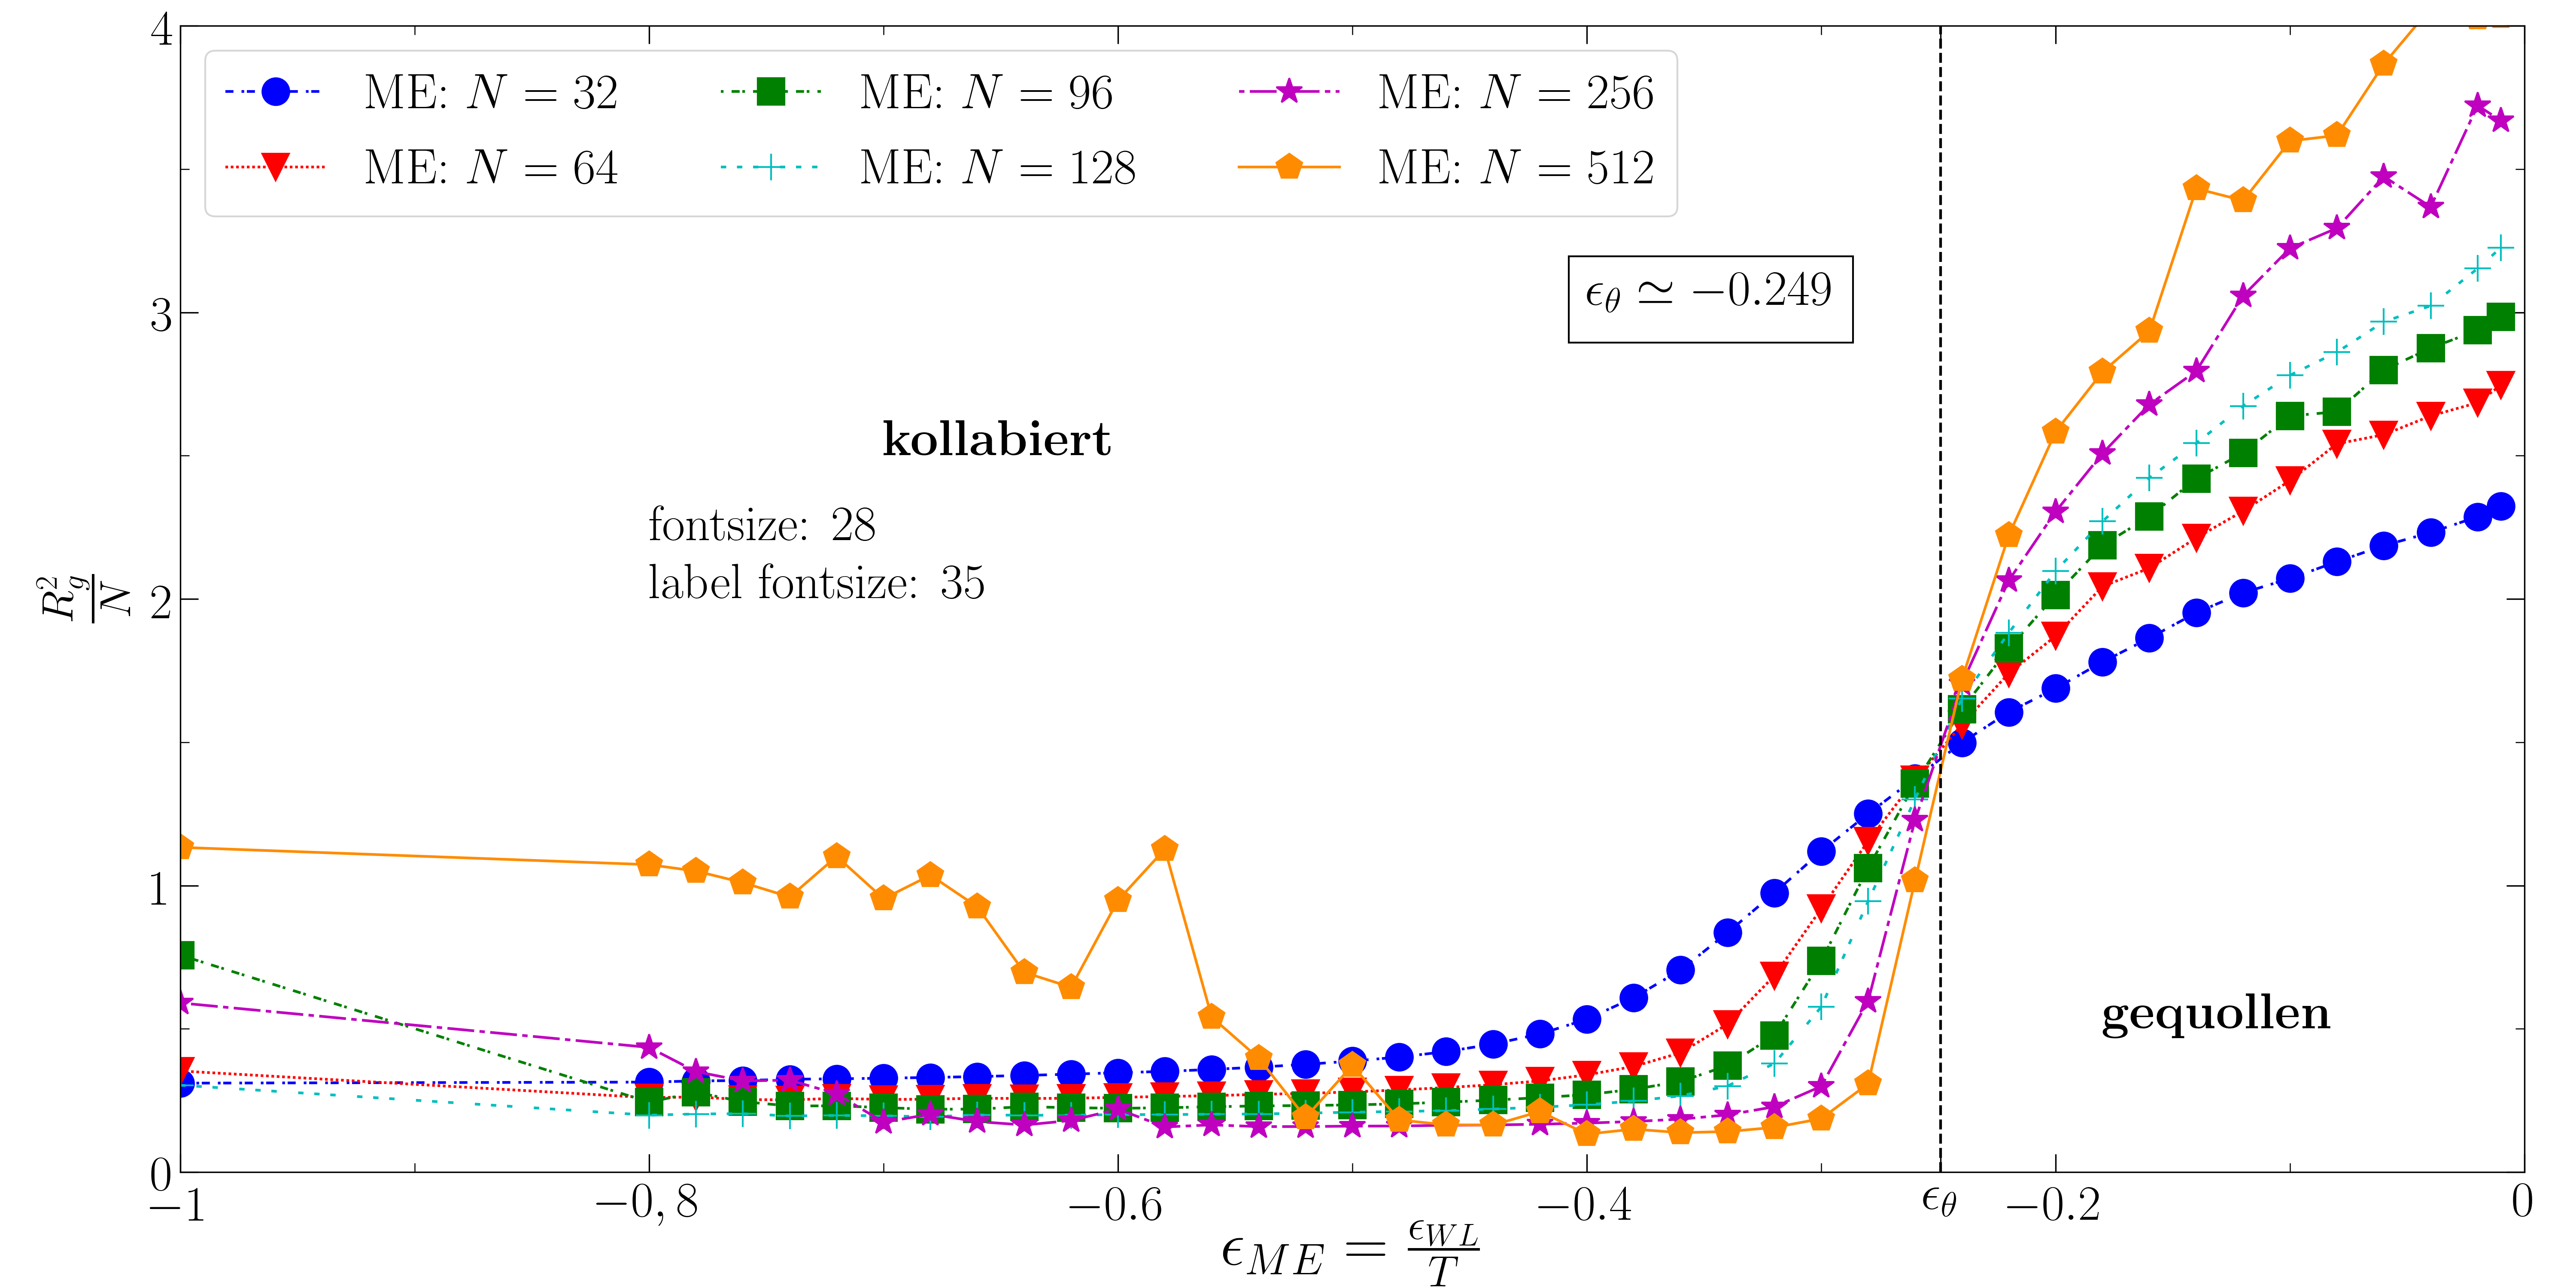
\includegraphics[width=\textwidth]{png_28_28.png}
\caption{Beschreibung des Bildes zum Größenvergleich mit der Schrift des Dokuments}
\end{figure}
Normale Schriftgröße im ganzen Dokument.
\begin{figure}[H]

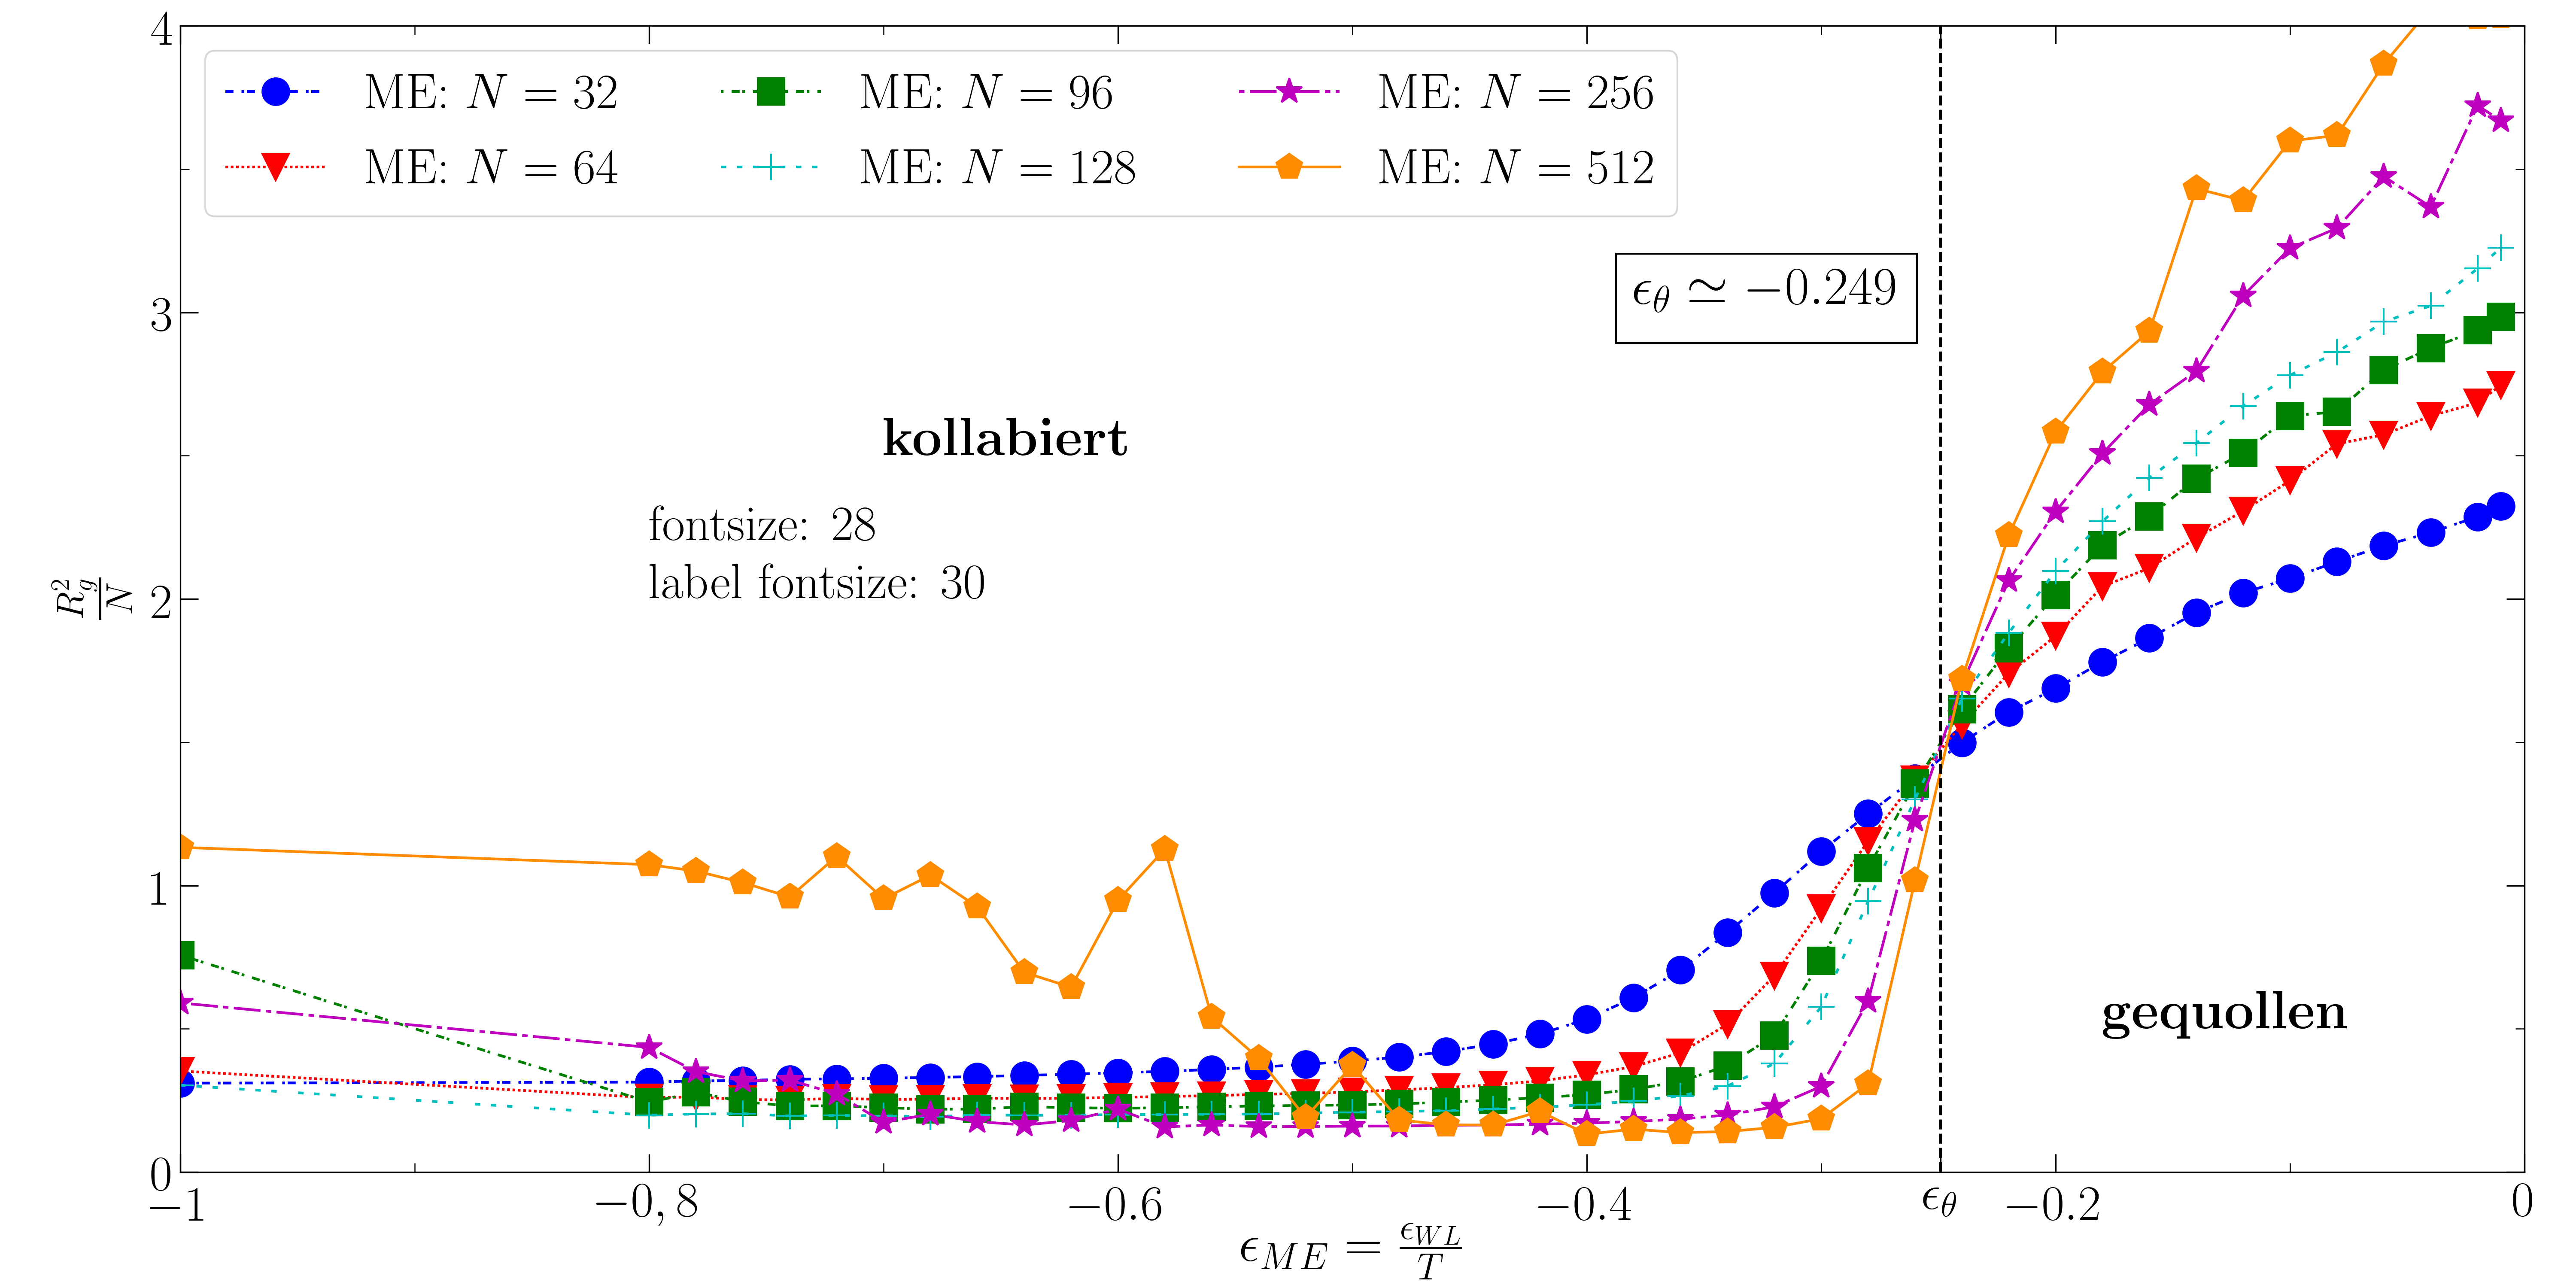
\includegraphics[width=\textwidth]{png_28_30.png}
\caption{Beschreibung des Bildes zum Größenvergleich mit der Schrift des Dokuments}
\end{figure}
Normale Schriftgröße im ganzen Dokument.
\begin{figure}[H]
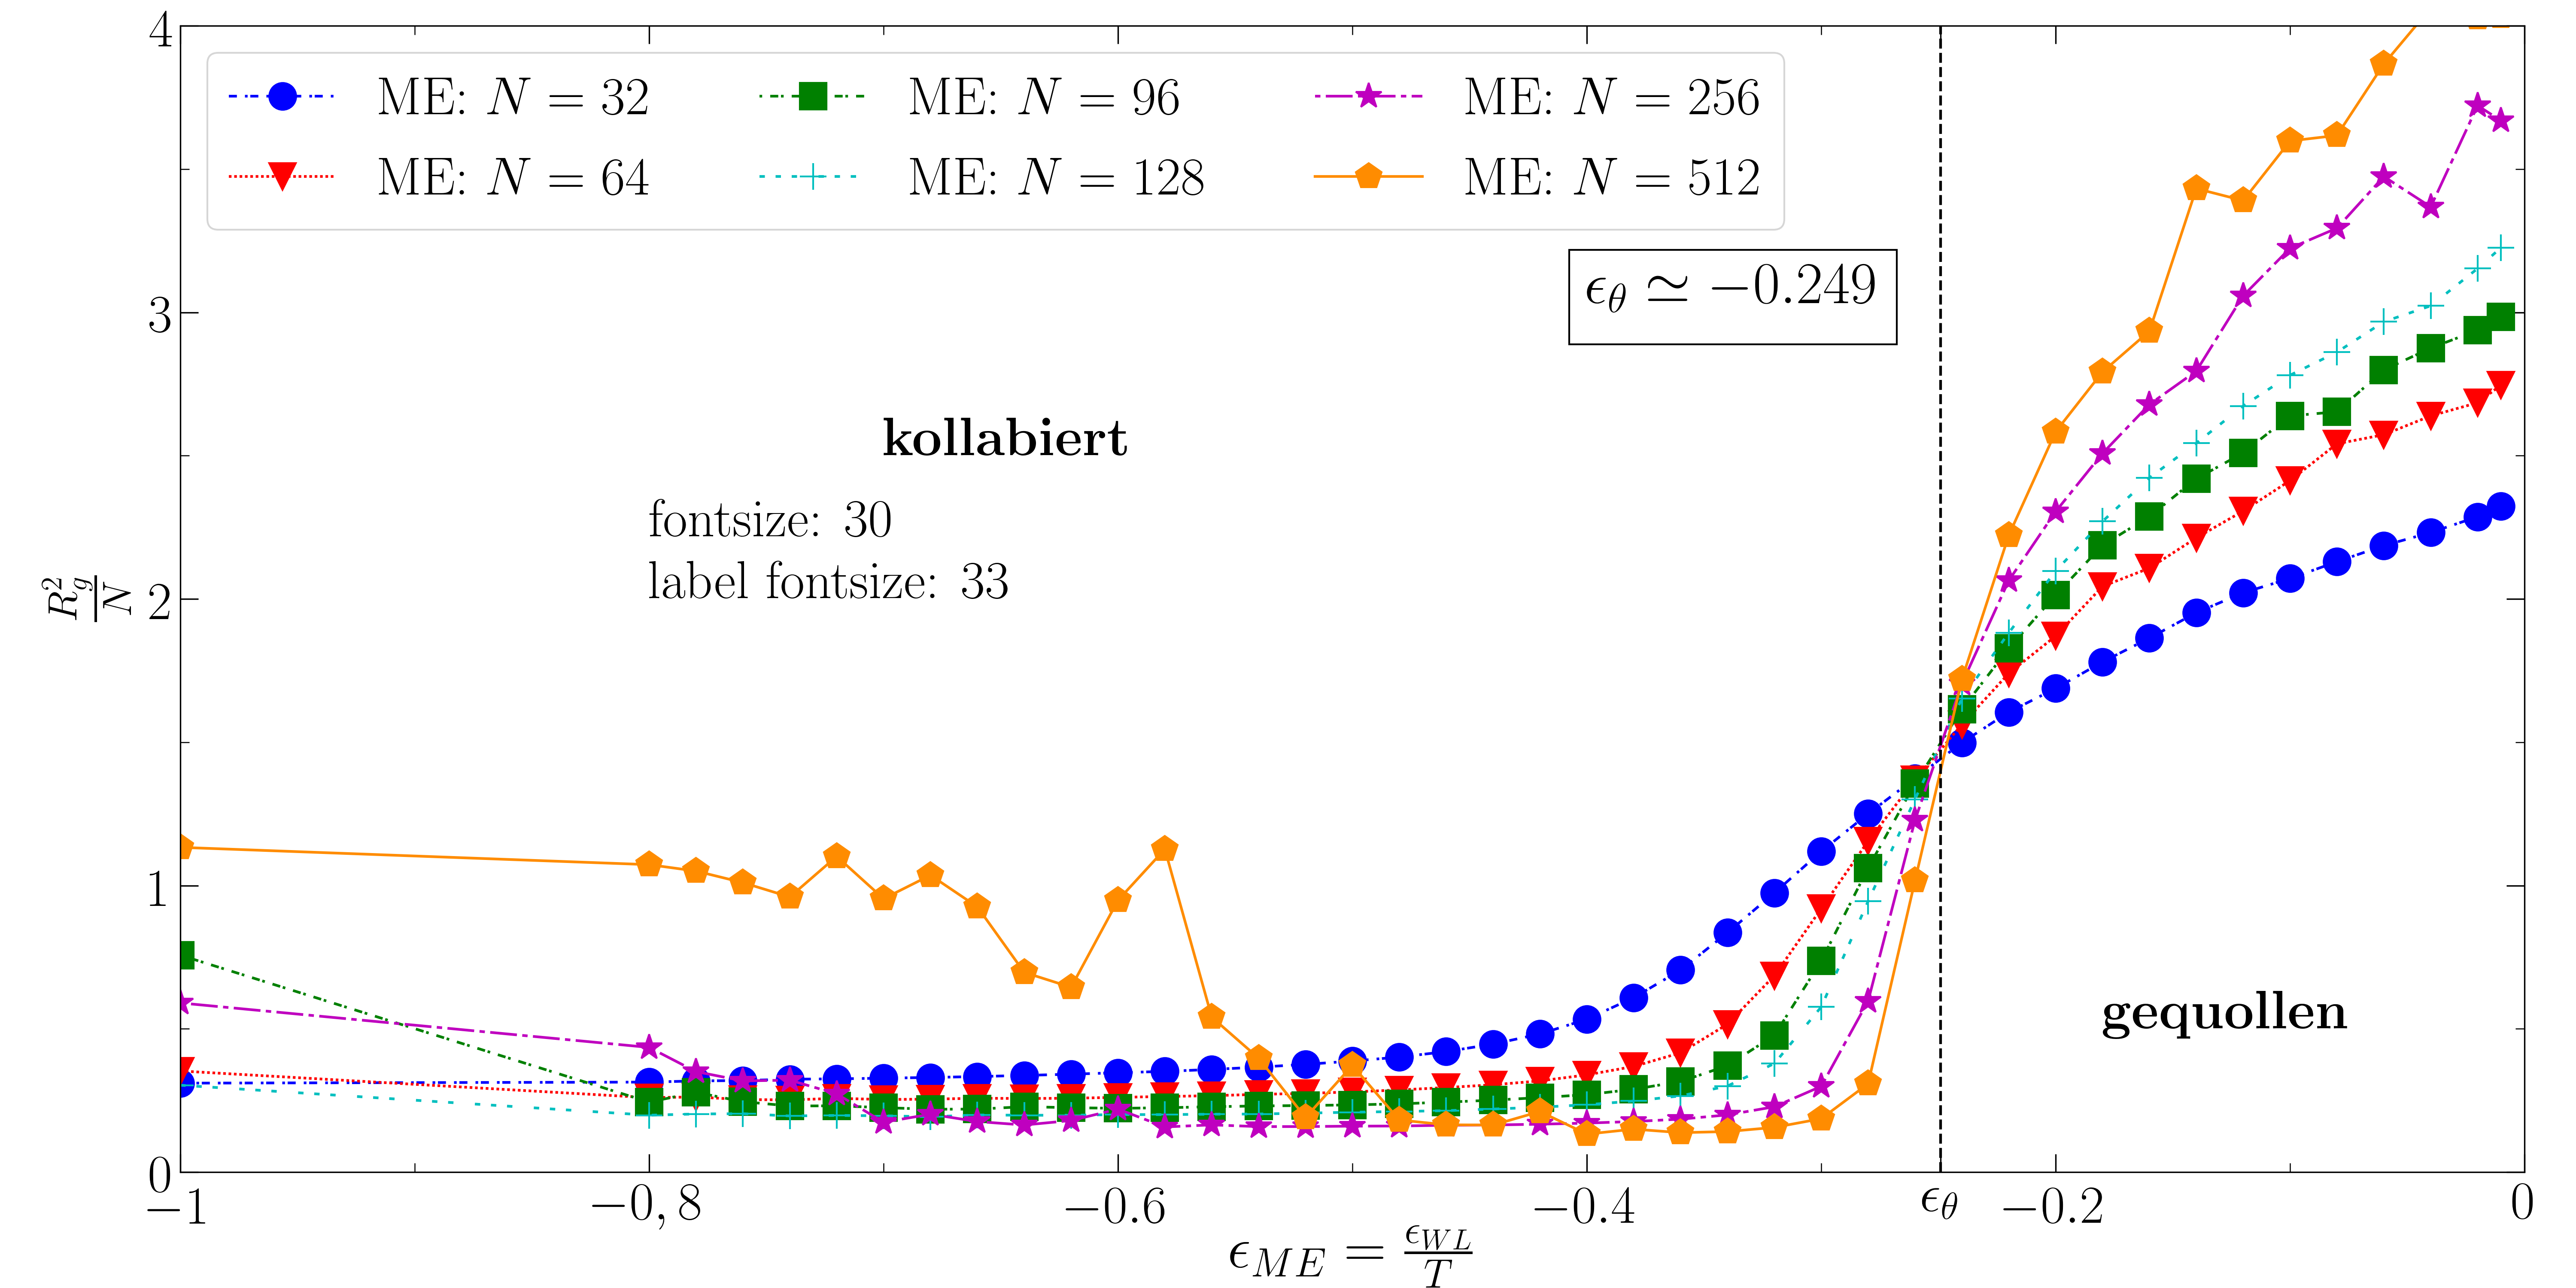
\includegraphics[width=\textwidth]{png_30_30.png}
\caption{Beschreibung des Bildes zum Größenvergleich mit der Schrift des Dokuments}
\end{figure}
Normale Schriftgröße im ganzen Dokument.
\begin{figure}[H]
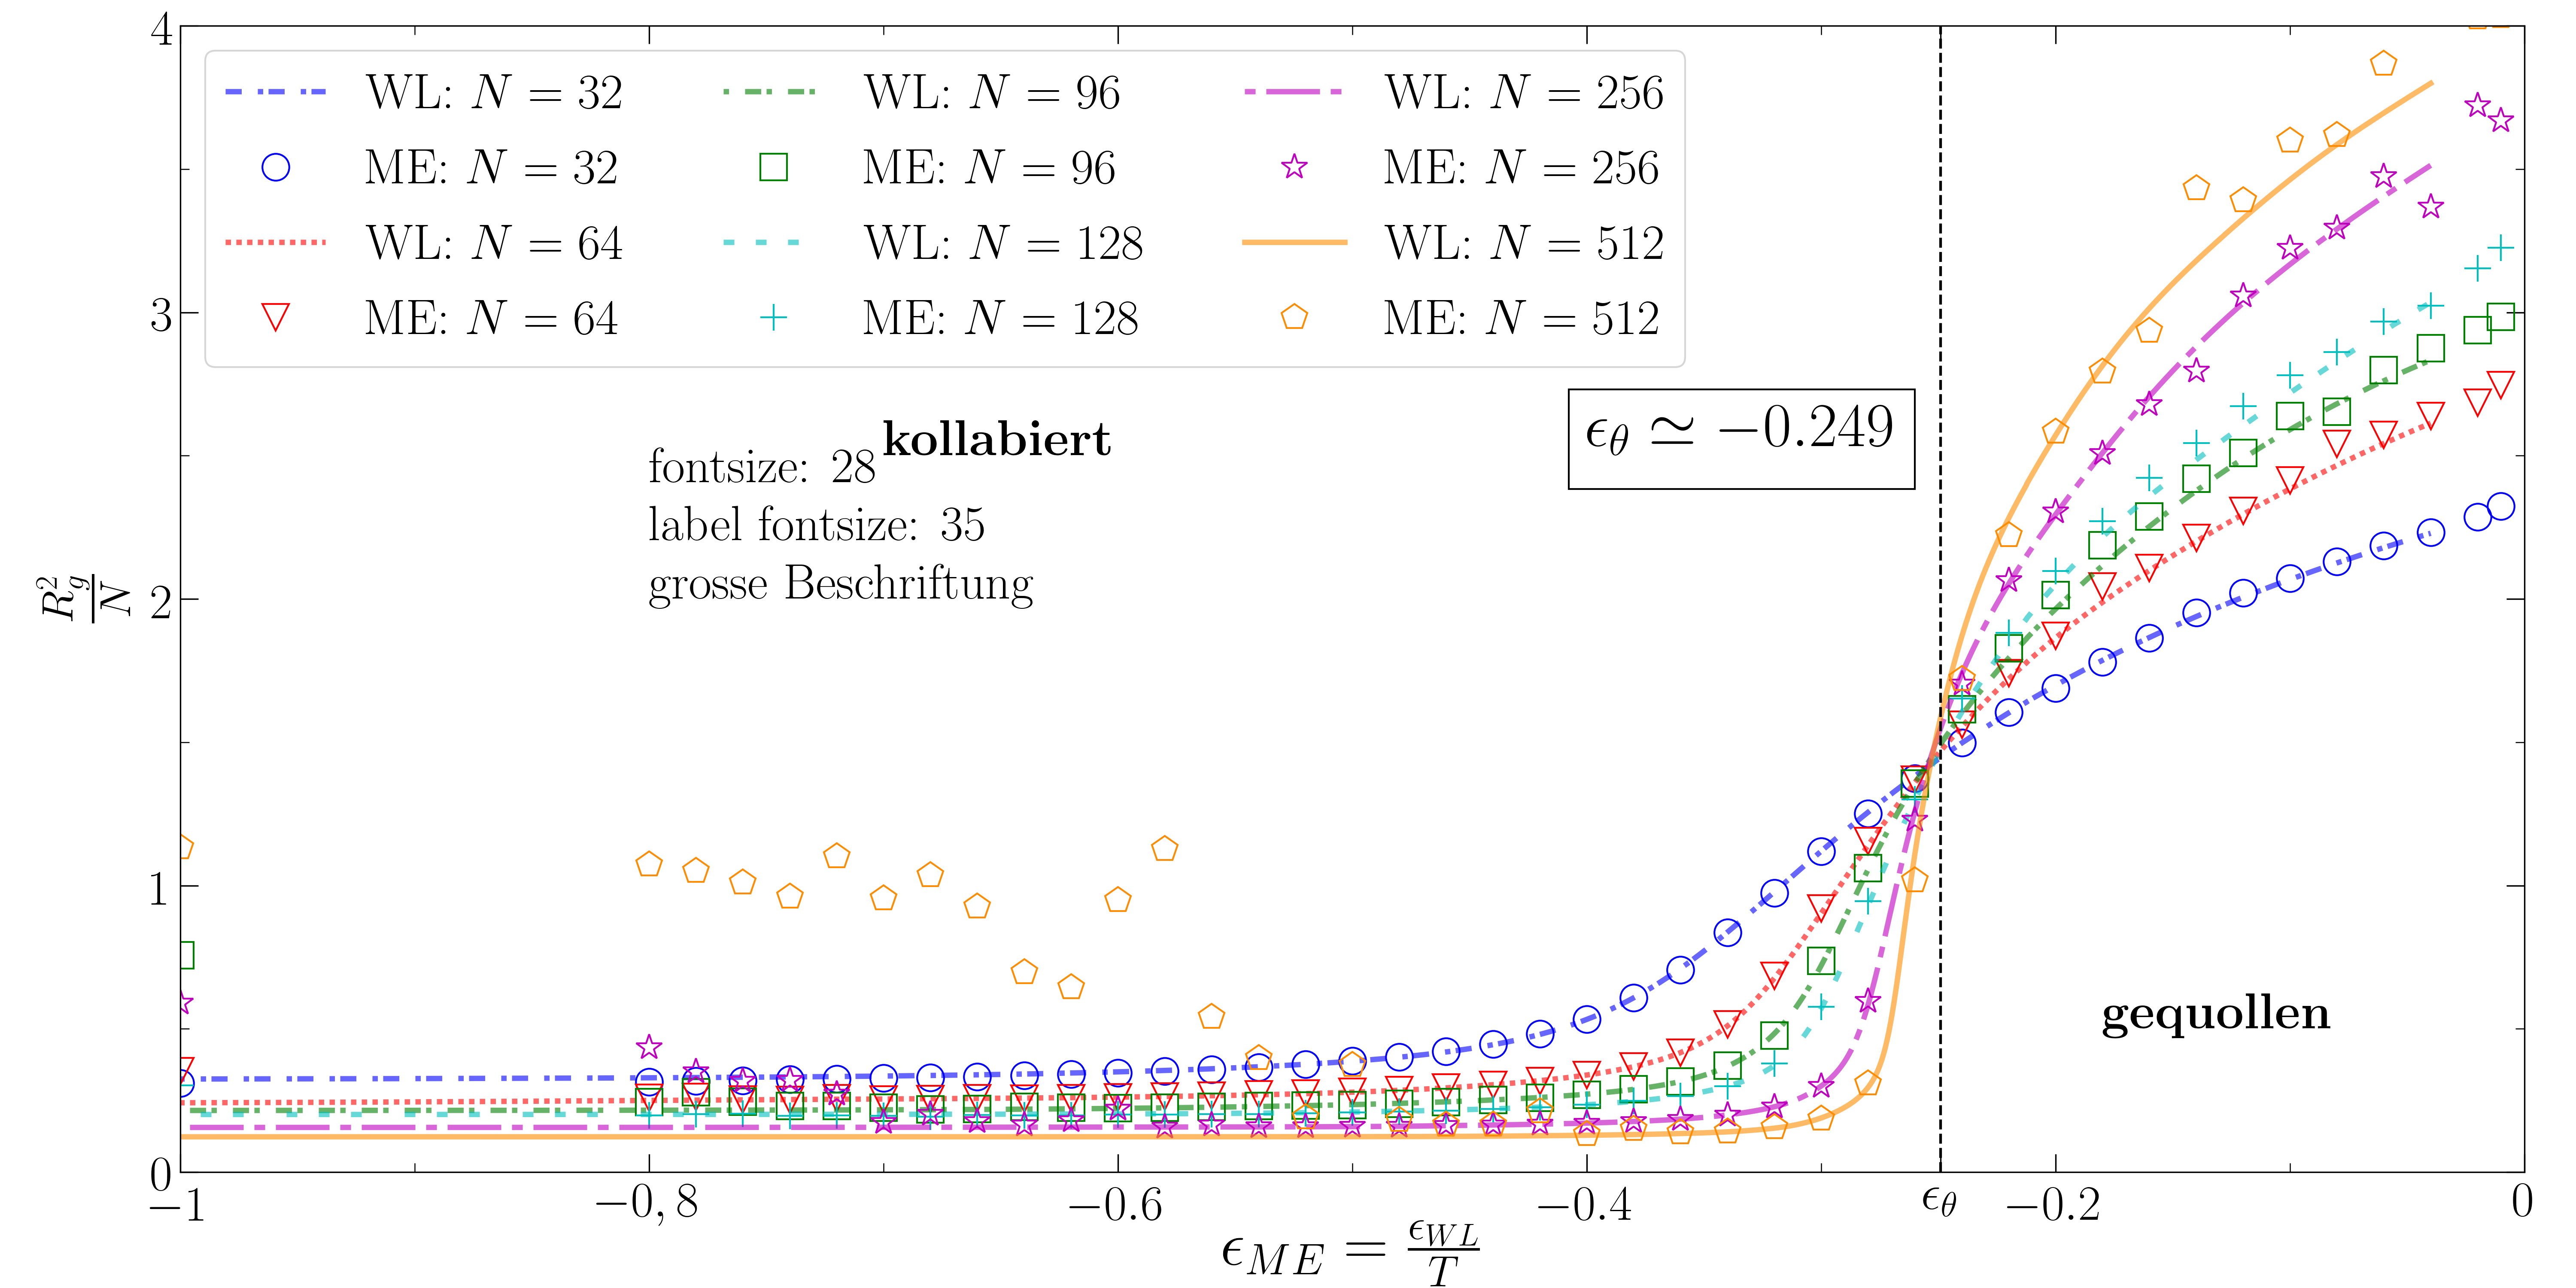
\includegraphics[width=\textwidth]{pngwl_28_28}
\caption{Beschreibung des Bildes zum Größenvergleich mit der Schrift des Dokuments}
\end{figure}
Normale Schriftgröße im ganzen Dokument.
\begin{figure}[H]
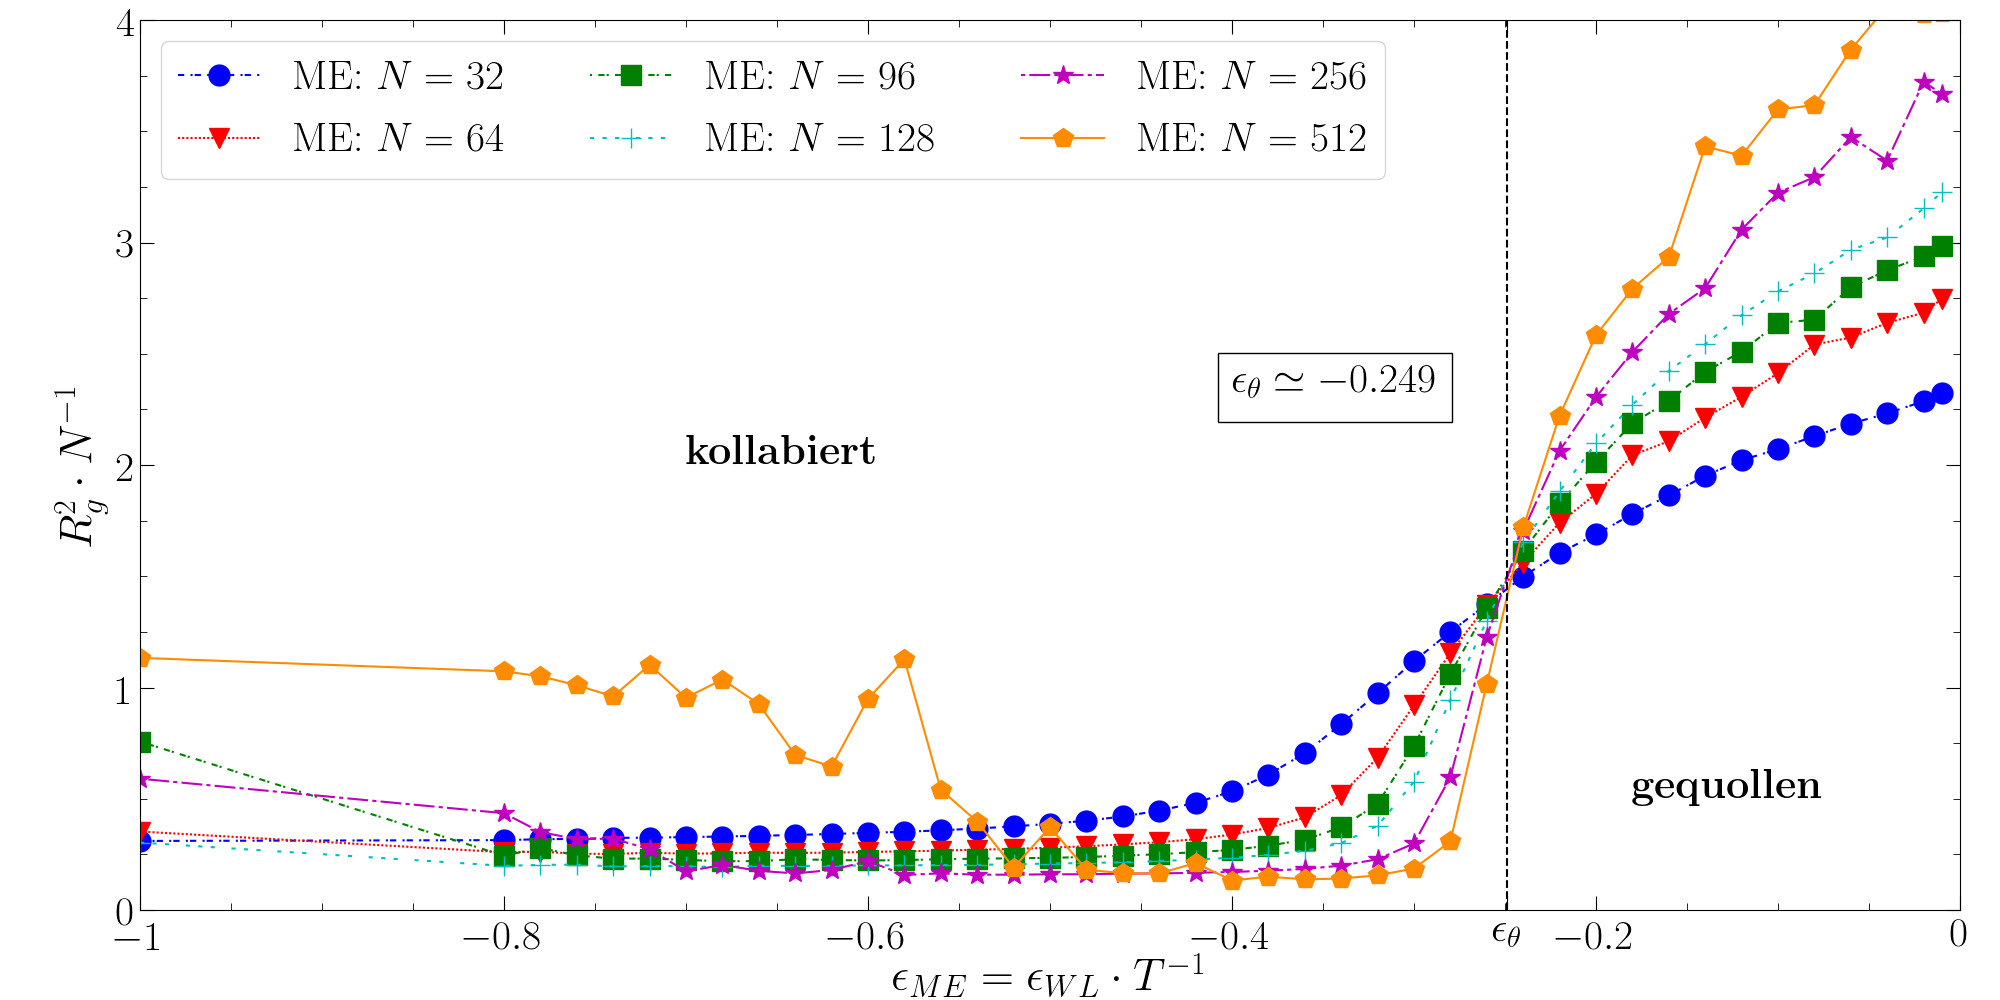
\includegraphics[width=\textwidth]{Vorschlag_Ron}
\caption{Eine Grafik mit Rons Vorschlägen}
\end{figure}
Normale Schriftgröße im ganzen Dokument.
\begin{figure}[H]
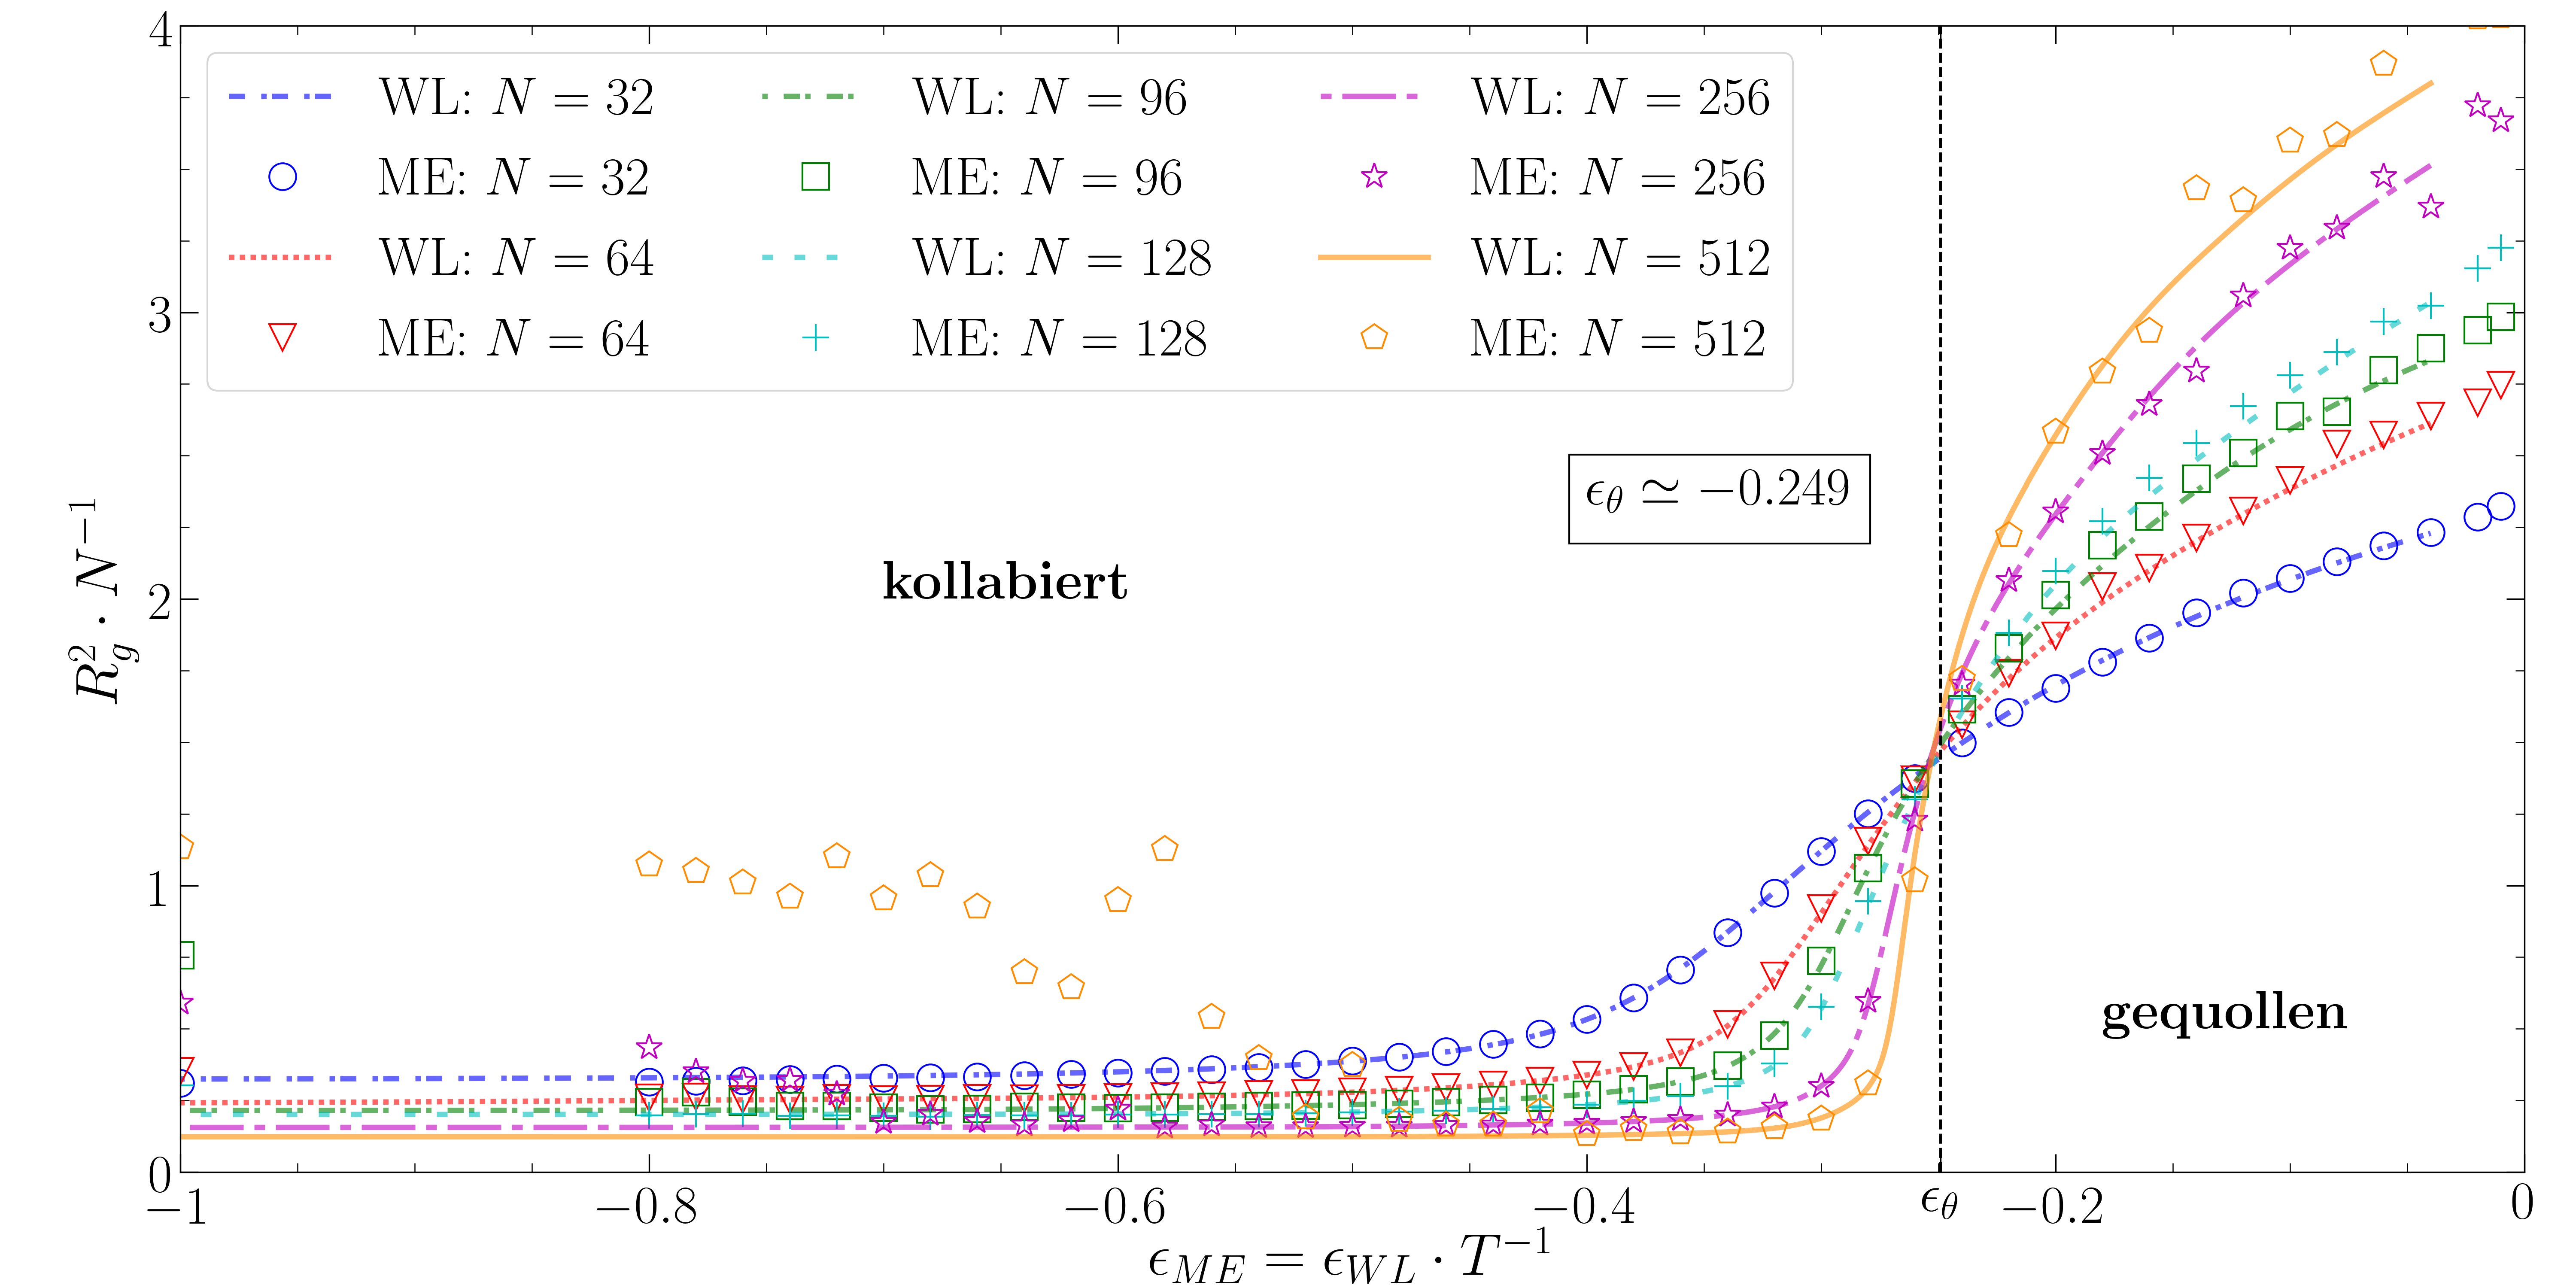
\includegraphics[width=\textwidth]{pngwl_30_33}
\caption{Eine Grafik mit den umgesetzen Vorschlägen Rons mit großer Legende.}
\end{figure}
Normale Schriftgröße im ganzen Dokument.


\end{document}



